% BrandShield AI - IEEE conference paper, first draft
% Compile on Overleaf: choose pdfLaTeX. Template: IEEEtran conference mode.
% TODO before submission: fill in author emails, add figures, verify every reference.

\documentclass[conference]{IEEEtran}
\IEEEoverridecommandlockouts

\usepackage{cite}
\usepackage{amsmath,amssymb,amsfonts}
\usepackage{algorithmic}
\usepackage{graphicx}
\usepackage{textcomp}
\usepackage{xcolor}
\usepackage{booktabs}
\usepackage{url}
\def\BibTeX{{\rm B\kern-.05em{\sc i\kern-.025em b}\kern-.08em T\kern-.1667em\lower.7ex\hbox{E}\kern-.125emX}}

\begin{document}

\title{BrandShield AI: A Real-Time Multilingual Pipeline for Aspect-Based
Brand Sentiment Analysis and Crisis Detection on Social Media}

\author{
\IEEEauthorblockN{Soham Borse, Tanish Bantwal, Aryan Baakle, Omsingh Rajput}
\IEEEauthorblockA{\textit{Dept. of Artificial Intelligence and Data Science} \\
\textit{K. K. Wagh Institute of Engineering Education and Research} \\
Nashik, Maharashtra, India \\
% TODO: add contact emails
}
\and
\IEEEauthorblockN{Dr. Darshan Medhane}
\IEEEauthorblockA{\textit{Dept. of Artificial Intelligence and Data Science} \\
\textit{K. K. Wagh Institute of Engineering Education and Research} \\
Nashik, Maharashtra, India \\
% TODO: add contact email
}
}

\maketitle

\begin{abstract}
Online brand reputation can deteriorate within hours, yet most organisations still
monitor social platforms manually or with tools that report sentiment only after the
fact. This paper presents BrandShield AI, an end-to-end system that ingests public
social-media conversation in real time, classifies it with a multilingual transformer,
decomposes opinion by aspect, and detects reputation crises before they escalate. The
system unifies four stages in one streaming pipeline: collection from YouTube,
Instagram, news feeds and app-store reviews through official APIs; a hybrid classifier
that averages two BERT-family encoders fine-tuned on social-media text (RoBERTa and
multilingual XLM-RoBERTa) and blends them with a code-mixed opinion lexicon and a
confidence-margin rule for the neutral class; clause-level aspect-based sentiment
analysis over a configurable aspect lexicon; and crisis detection that couples an
Isolation Forest over time-bucketed features with an adaptive median/MAD threshold on
the negative share, followed by Prophet-based forecasting and a five-signal risk score.
On a hand-labelled multilingual benchmark of 83 brand comments spanning English,
Hinglish, Hindi and Marathi, the hybrid classifier reaches 83.1\% accuracy and 81.7\%
macro-F1, and aspect detection attains $F_1 = 0.806$. On 200 real comments sampled at random
from the live system it reaches 74.0\% accuracy, against 66.5\% for the DistilBERT
model we first deployed---a gap our team-written benchmark had hidden. Against an
independent external signal---483 App Store reviews with user-assigned star
ratings---predictions agree 79.7\% of the time. The deployed system analysed
12{,}174 real comments on commodity CPU hardware with no GPU. In a controlled crisis experiment the detector raised its first
alert 24\,s after a negative-sentiment surge began, driving the brand-risk score from 20 to
79 out of 100.
\end{abstract}

\begin{IEEEkeywords}
brand reputation management, sentiment analysis, aspect-based sentiment analysis,
BERT, RoBERTa, XLM-RoBERTa, anomaly detection, Isolation Forest, time-series forecasting, code-mixed
text, real-time systems
\end{IEEEkeywords}

\section{Introduction}

Social platforms have become the primary channel through which customers express
satisfaction and dissatisfaction with brands. A single complaint can reach millions of
viewers within hours, and the window in which an organisation can respond effectively is
correspondingly short. Traditional reputation monitoring---staff reading mentions
manually, or dashboards that summarise sentiment retrospectively---is poorly matched to
this timescale.

Three limitations recur in existing practice. First, most deployed tools report
\emph{polarity} but not \emph{cause}: knowing that 30\% of mentions are negative does not
tell a manager whether the problem is delivery, pricing or product quality. Second,
commercial monitoring suites are priced for large enterprises, placing them out of reach
of the small and medium businesses most exposed to a viral complaint. Third, sentiment
models are typically trained and evaluated on monolingual English corpora, whereas real
conversation in markets such as India is heavily code-mixed, with Hinglish and
Devanagari-script comments appearing alongside English in the same thread.

This paper describes BrandShield AI, built to address these gaps simultaneously. The
contributions are:

\begin{enumerate}
\item A complete streaming architecture in which collection, natural-language
processing, analytics and alerting are decoupled through a message bus, so that a slow or
rate-limited platform API degrades without stalling classification.
\item A hybrid sentiment classifier that averages two BERT-family encoders fine-tuned on
tweets (RoBERTa and XLM-RoBERTa) and augments them with a Hinglish, Hindi and Marathi
opinion lexicon and a confidence-margin rule for the neutral class, evaluated both on a
team-written benchmark and on randomly sampled real comments.
\item Clause-level aspect-based sentiment analysis driven by a user-editable aspect
lexicon, so that a mixed opinion contributes positively to one aspect and negatively to
another.
\item A two-signal crisis detector combining an unsupervised Isolation Forest with a
robust median/MAD z-score computed on the \emph{share} of negative mentions rather than
their raw count, which removes the false positives that daily traffic seasonality
otherwise induces.
\item An evaluation on real data, including an external validity check against
user-assigned star ratings and a controlled crisis-injection experiment that measures
detection latency end to end.
\end{enumerate}

The system runs without a GPU: the complete pipeline occupies about 2\,GB of
resident memory and classifies a comment in 32--120\,ms on a laptop CPU, making deployment
on a commodity virtual machine practical.

\section{Related Work}

\textbf{Transformer-based sentiment classification.} BERT~\cite{devlin2019bert}
established fine-tuned bidirectional transformers as the standard approach to
sentence-level sentiment classification. DistilBERT~\cite{sanh2019distilbert} reduces
parameters by approximately 40\% and increases inference speed by approximately 60\%
while retaining most of the accuracy. RoBERTa~\cite{liu2019roberta} keeps the BERT
architecture but improves pre-training, and XLM-RoBERTa~\cite{conneau2020xlmr} extends it to
100 languages; Cardiff NLP fine-tuned both on tweets~\cite{barbieri2022xlmt,loureiro2022timelms},
which matters for short, informal, emoji-heavy comments.

\textbf{Lexicon and hybrid methods.} VADER~\cite{hutto2014vader} is a rule- and
lexicon-based analyser tuned for social media that remains competitive on short informal
text at a fraction of transformer cost. Our work differs in \emph{where} the lexicon is
applied: rather than ensembling two general-purpose classifiers, we use a narrow lexicon
restricted to romanised Indian-language opinion words, applied as a corrective prior
where the multilingual transformer is weakest.

\textbf{Code-mixed sentiment.} Sentiment analysis of Hindi--English code-mixed text is an
established sub-problem~\cite{joshi2016subword,patwa2020semeval}, with shared tasks
demonstrating that models trained on monolingual corpora degrade substantially on
romanised, transliterated input. This motivates the lexicon component of our classifier.

\textbf{Aspect-based sentiment analysis.} The SemEval ABSA tasks~\cite{pontiki2014semeval}
formalised extraction of aspect terms and their polarities. Fully supervised neural ABSA
requires aspect-annotated training data, unavailable for an arbitrary brand's vocabulary.
We adopt a lightweight lexicon-and-clause approach that a non-technical user can extend
at runtime, trading recall for zero annotation cost and immediate configurability.

\textbf{Anomaly detection and forecasting.} Isolation Forest~\cite{liu2008isolation}
isolates anomalies through random partitioning and suits unlabelled, low-dimensional
telemetry such as per-interval mention statistics. Prophet~\cite{taylor2018forecasting}
provides decomposable trend-and-seasonality forecasting that is robust to missing data
and interpretable by non-specialists. Our contribution is their combination with a
direction-aware adaptive threshold inside a single risk score.

\textbf{Research gap.} Prior systems typically deliver sentiment classification
\emph{or} forecasting \emph{or} anomaly detection. Few integrate aspect-level attribution
with crisis detection in a live pipeline, and fewer still are evaluated on code-mixed
Indian-language brand conversation.

\section{System Architecture}

The system is organised in six layers (Fig.~\ref{fig:arch}).

\begin{figure}[t]
\centerline{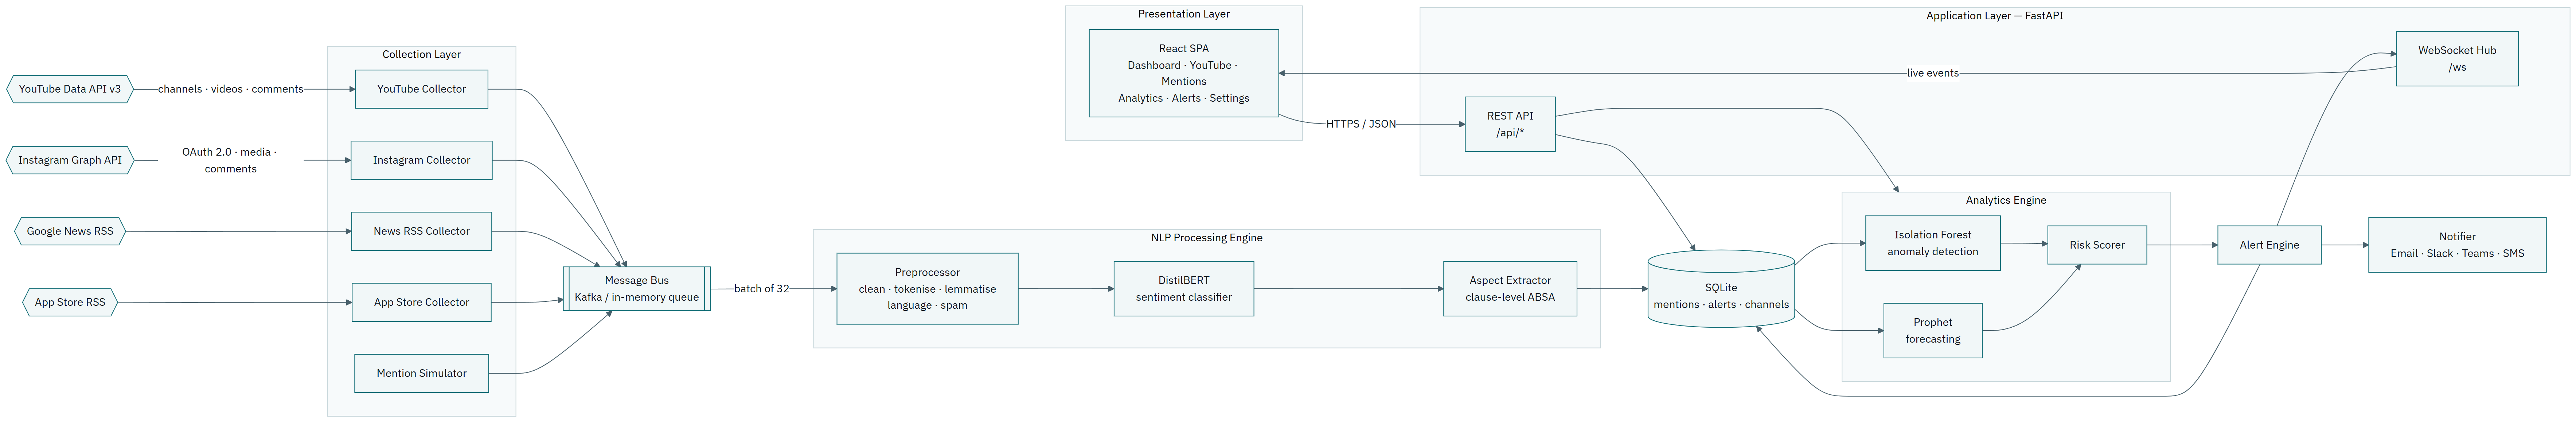
\includegraphics[width=\columnwidth]{fig1_architecture.png}}
\caption{Layered architecture of BrandShield AI. Collectors publish to a message bus, decoupling platform APIs from classification; analytics and alerting consume persisted results.}
\label{fig:arch}
\end{figure}

\textbf{Collection layer.} Five collectors implement a common interface
(\texttt{configured()}, \texttt{status()}, \texttt{poll()}) and are polled on independent
schedules: YouTube every 300\,s, Instagram every 180\,s, news and app-store feeds every
180\,s. Adding a platform requires implementing the interface only. All access is
read-only through official APIs: the YouTube Data API v3, the Instagram API with
Instagram Login (OAuth 2.0 with user consent), Google News RSS and the Apple App Store
customer-review RSS feed.

\textbf{Streaming layer.} Collectors publish to a message bus rather than calling the
classifier directly. Two interchangeable implementations sit behind one interface: Apache
Kafka~\cite{kreps2011kafka} for distributed deployment and an in-process asynchronous
queue for single-node deployment. An API stall or a burst of several thousand comments
therefore changes queue depth rather than blocking ingestion.

\textbf{NLP processing layer.} A consumer drains the bus in batches of up to 32 messages
and applies preprocessing, sentiment classification and aspect extraction before
persisting results.

\textbf{Analytics layer.} Every 30\,s the system aggregates stored mentions into fixed
time buckets, scores them for anomalies and recomputes the brand-risk score; forecasts
refresh every 5\,min.

\textbf{Alerting layer.} Six rules convert analytic state into alerts, each with a
cool-down to prevent duplicates. Alerts are pushed to dashboards over WebSocket and
optionally to email, Slack, Microsoft Teams or SMS.

\textbf{Presentation layer.} A React single-page application renders live dashboards;
updates arrive by WebSocket push rather than polling.

\section{Methodology}

\subsection{Preprocessing}

Each mention passes through a deterministic pipeline: removal of URLs, @-mentions and
HTML; hashtag unwrapping; collapsing of character runs (\emph{sooooo} $\rightarrow$
\emph{soo}); mapping of 30 frequent emoji to lexical equivalents, since the tokenizer
represents most emoji as unknown tokens; tokenisation; stop-word removal with negation
terms explicitly retained; WordNet lemmatisation; and language identification. A
rule-based spam filter flags promotional and bot content using pattern families
(follower-exchange phrases, link-heavy posts, hashtag stuffing, all-caps with links).
Spam is stored but excluded from sentiment statistics.

\subsection{Hybrid Sentiment Classification}

The base classifier averages two BERT-family encoders fine-tuned on tweets:
XLM-RoBERTa (multilingual) and RoBERTa (English). Each yields a distribution over
positive, neutral and negative; let $p_m = (p^+, p^0, p^-)$ denote their mean. If neither
model can be loaded, a multilingual DistilBERT with five ordinal classes, folded into
three, is used as a fallback.

For code-mixed input we compute a lexicon polarity $\ell \in [-1,1]$ as the mean signed
weight of matched opinion terms from a curated Hinglish, Hindi and Marathi lexicon, with
negation inversion inside a $\pm 2$-token window. When at least one term matches, the
distributions are blended:
\begin{equation}
p = (1-\lambda)\,p_m + \lambda\,p_\ell, \qquad \lambda = 0.35
\end{equation}
where $p_\ell = (\max(\ell,0),\, 1-|\ell|,\, \max(-\ell,0))$.

A neutral-margin rule then addresses the model's tendency to assign weak polarity to
factual statements. Let $p_{(1)} \ge p_{(2)}$ be the two largest class probabilities. If
the top class is not neutral, no lexicon term matched, and
\begin{equation}
p_{(1)} - p_{(2)} < \delta, \qquad \delta = 0.20
\end{equation}
the prediction is reassigned to neutral. A continuous sentiment score
$s = p^+ - p^- \in [-1,1]$ is the quantity aggregated in all downstream analytics.
Predictions are cached by normalised text, which matters because social streams contain
many repeated and near-duplicate comments.

\subsection{Aspect-Based Sentiment Analysis}

Each mention is split into clauses at sentence delimiters and contrastive conjunctions
(\emph{but}, \emph{however}, \emph{lekin}, \emph{magar}, \emph{par}). Aspects are detected
per clause by whole-word matching against a configurable lexicon of eight default aspects
(food quality, service, delivery, price, ambience, hygiene, app experience, packaging);
whole-word matching avoids substring errors such as \emph{late} inside \emph{chocolate}.
Each aspect-bearing clause is classified independently by the same sentiment model, so a
mixed opinion yields opposite polarities for different aspects. Users may add, remove or
extend aspects at runtime without redeployment.

\subsection{Crisis Detection}

Mentions are aggregated into fixed $b$-minute buckets ($b=15$ by default). For each bucket
we compute total volume $n_t$, per-class counts, mean sentiment $\bar{s}_t$ and the
negative share $r_t = n^-_t / n_t$.

Two detectors run in parallel. An Isolation Forest~\cite{liu2008isolation} is fitted over
the trailing window using the feature vector
$\langle n_t, n^-_t, r_t, \bar{s}_t, \Delta n^-_t \rangle$, with anomaly scores normalised
to $[0,1]$. In parallel a robust z-score is computed against a trailing baseline using the
median and median absolute deviation:
\begin{equation}
z_t = \frac{x_t - \operatorname{med}(x_{t-w:t-1})}
{1.4826 \cdot \operatorname{MAD}(x_{t-w:t-1})}
\end{equation}

A bucket is flagged only when the anomaly is \emph{harmful}---that is, when the negative
share deviates upward, confirmed by the negative count:
\begin{align}
\mathrm{crisis}_t = {} & (n^-_t \ge n_{\min}) \wedge \big[ \notag \\
& \big(\mathrm{IF}_t \wedge z^r_t \ge \tau \wedge z^{n^-}_t \ge 0.6\tau\big) \vee \notag \\
& \big(z^r_t \ge 1.6\tau \wedge z^{n^-}_t \ge \tau\big) \big]
\end{align}
with $\tau = 2.5$ and $n_{\min} = 5$. Using the negative \emph{share} as the primary
signal is the design decision that makes the detector usable: raw negative counts rise
every day at lunch and evening peaks, and a count-based threshold flags those normal peaks
as crises (Section~\ref{sec:crisis}).

\subsection{Forecasting and Risk Scoring}

Hourly series of mean sentiment, negative share and volume are forecast with
Prophet~\cite{taylor2018forecasting}; with fewer than 36 hourly observations, or when
Prophet fails to converge, the system falls back to Holt linear smoothing with an
empirical prediction interval.

The brand-risk score $R \in [0,100]$ combines five bounded components:
\begin{equation}
R = 35 f_1 + 20 f_2 + 25 f_3 + 10 f_4 + 10 f_5
\end{equation}
where $f_1$ measures the recent negative share and its lift over baseline (negativity),
$f_2$ the negative-count z-score (velocity), $f_3$ the Isolation Forest score when a
bucket is flagged (anomaly), $f_4$ the forecast decline over the next six hours, and
$f_5$ the share of complaints attributable to a single aspect (concentration). Scores map
to four levels---low, medium, high, critical. Requiring several independent signals to
coincide before a high score is reported is what suppresses single-signal false alarms. A
complementary brand-health index $H = 50 + 50\bar{s}$ is reported for readability.

\subsection{Alerting}

Six rules raise alerts: negative spike, risk threshold crossed, sustained negative ratio,
aspect surge, forecast decline, spam wave, and virality of an individual negative post.
Each rule carries a deduplication key and cool-down (default 30\,min), so one incident
produces one alert rather than a stream.

\section{Experimental Setup}

\subsection{Hardware and Software}

\begin{table}[htbp]
\caption{Experimental and deployment environment}
\label{tab:hw}
\centering
\begin{tabular}{@{}lll@{}}
\toprule
\textbf{Component} & \textbf{Development} & \textbf{Deployment (min.)} \\
\midrule
Processor & Ryzen 7 7435HS, 8C/16T & 2 vCPU x86-64 \\
Memory    & 24\,GB                 & 4\,GB (2\,GB used) \\
Storage   & SSD                    & 25\,GB (1.6\,GB models) \\
GPU       & RTX 4050 (unused)      & none required \\
OS        & Windows 11             & Ubuntu 24.04 LTS \\
\bottomrule
\end{tabular}
\end{table}

Software: Python 3.14, FastAPI 0.141, PyTorch 2.14 (CPU build), Transformers 5.17,
scikit-learn 1.9.1, Prophet 1.4, NLTK 3.10, pandas 3.0.5 and SQLite 3; React 19 with
Chart.js 4.5 for the interface.

\subsection{Datasets}

\textbf{D1---Annotated benchmark (83 comments).} Brand comments hand-labelled as
positive, neutral or negative, deliberately constructed to include English, Hinglish,
romanised and Devanagari Hindi, Marathi, sarcasm, mixed opinions and spam. Aspect labels
accompany 47 comments. The set is small and single-annotator, which we treat as a
limitation.

\textbf{D2---Live corpus (12{,}174 mentions).} Collected by the deployed system: 11{,}063
YouTube comments, 135 Instagram comments, 491 Google News articles, 483 Apple App Store
reviews and 2 rows imported from CSV. Language identification reports English alongside
Indonesian, Spanish, Portuguese, Italian and Arabic, confirming that multilingual
capability is required in practice.

\textbf{D4---Real-comment benchmark (200 comments).} Comments sampled at random from the live
database (110 YouTube, 60 Instagram, 30 news) and labelled by hand: 47 negative, 91 neutral,
62 positive. Unlike D1, they were neither written nor selected by the team.

\textbf{D3---External validation (483 reviews).} App Store reviews carry a user-assigned
1--5 star rating, mapped to three classes (1--2 negative, 3 neutral, 4--5 positive) and
treated as an independent label produced by the reviewer rather than the research team.

\section{Results and Discussion}

\subsection{Sentiment Classification and Ablation}

\begin{table}[htbp]
\caption{Classification performance on D1 ($n = 83$) and D4 ($n = 200$)}
\label{tab:overall}
\centering
\begin{tabular}{@{}lccccc@{}}
\toprule
\textbf{Configuration} & \textbf{Acc.} & \textbf{P} & \textbf{R} & \textbf{F1} & \textbf{F1$_w$} \\
\midrule
\multicolumn{6}{@{}l}{\emph{D1, team-written benchmark}} \\
DistilBERT only  & 0.7831 & 0.7735 & 0.7595 & 0.7647 & 0.7815 \\
DistilBERT hybrid & 0.7831 & 0.7838 & 0.7738 & 0.7764 & 0.7870 \\
Ensemble only & 0.8072 & 0.7918 & 0.7952 & 0.7904 & 0.8124 \\
Ensemble hybrid (deployed) & \textbf{0.8313} & \textbf{0.8174} & \textbf{0.8238} & \textbf{0.8174} & \textbf{0.8352} \\
\midrule
\multicolumn{6}{@{}l}{\emph{D4, random real comments}} \\
DistilBERT hybrid & 0.6650 & -- & -- & 0.6520 & -- \\
Ensemble hybrid (deployed) & \textbf{0.7400} & \textbf{0.7844} & \textbf{0.7050} & \textbf{0.7276} & \textbf{0.7362} \\
\bottomrule
\end{tabular}
\end{table}

On D1 the lexicon-and-margin layer adds 2.4 points of accuracy and 2.7 points of
macro-F1 to the ensemble; the transformer does most of the work and the lexicon corrects a
specific, identifiable failure mode. The more consequential finding is the D1--D4 gap for
DistilBERT: 78.3\% on the team-written benchmark but 66.5\% on random real comments, where
fan slang, emoji-only replies and non-English comments dominate its errors. The ensemble
narrows this gap (83.1\% and 74.0\%). An earlier candidate model reached only 49.4\%
accuracy on D1, so model selection---validated on unselected real data rather than on
benchmarks alone---accounted for the largest improvements in this project.

\subsection{Per-Class Performance}

\begin{table}[htbp]
\caption{Per-class performance of the deployed classifier on D1}
\label{tab:perclass}
\centering
\begin{tabular}{@{}lcccc@{}}
\toprule
\textbf{Class} & \textbf{Precision} & \textbf{Recall} & \textbf{F1} & \textbf{Support} \\
\midrule
Negative & 0.967 & 0.829 & 0.892 & 35 \\
Neutral  & 0.652 & 0.750 & 0.698 & 20 \\
Positive & 0.833 & 0.893 & 0.862 & 28 \\
\bottomrule
\end{tabular}
\end{table}

\begin{table}[htbp]
\caption{Confusion matrix (rows: true, columns: predicted)}
\label{tab:cm}
\centering
\begin{tabular}{@{}lccc@{}}
\toprule
 & \textbf{Negative} & \textbf{Neutral} & \textbf{Positive} \\
\midrule
Negative & 29 & 5  & 1  \\
Neutral  & 1  & 15 & 4  \\
Positive & 0  & 3  & 25 \\
\bottomrule
\end{tabular}
\end{table}

Only one of 35 negative comments on D1 (and two of 47 on D4) was classified as positive,
and negative precision is 0.97 on D1 and 0.87 on D4, so the system rarely reports a
satisfied customer where a dissatisfied one exists---the error direction that matters for a
reputation-monitoring tool. The commoner error on real data is a mild complaint labelled
neutral (19 of 47 negatives on D4). The neutral class is weakest on D1 ($F_1 = 0.698$),
consistent with the difficulty of separating factual statements from mild opinion.

\subsection{Aspect Detection}

Against the aspect-annotated subset of D1, lexicon-based aspect detection achieves
precision 0.900, recall 0.730 and $F_1 = 0.806$. Precision substantially exceeds recall,
which is the desirable asymmetry here: an aspect attributed to a complaint is almost
always correct, while some complaints are recorded without an aspect. Recall is bounded by
vocabulary coverage, and the lexicon is user-extensible for exactly this reason.

\subsection{External Validation Against Star Ratings}

On D3, predictions agree with reviewer-assigned star ratings for 385 of 483 reviews
(79.7\%). Because these labels are produced by the reviewers themselves and were never
seen during development, this is an independent check that the accuracy measured on D1 is
not an artefact of the annotation process.

\subsection{Throughput and Latency}

Measured on the development CPU with batches of 32, the two-model ensemble needs
32.4\,ms per comment on D1 and 120\,ms on the longer D4 comments, about three times
DistilBERT's cost; single-comment interactive requests complete in approximately
140\,ms including HTTP overhead. The full pipeline occupies about
2\,GB resident memory. The system processed a backlog of more than
10{,}000 YouTube comments without a GPU, and repeated synchronisation of unchanged videos issues
zero additional comment-API calls---a quota optimisation without which the daily free
quota would be exhausted within hours.

\subsection{Crisis Detection}
\label{sec:crisis}

\textbf{Controlled experiment.} In a controlled test, we injected a burst of delivery complaints into the live stream using the crisis simulator, on top of the real data. The first alert, (\emph{sudden spike in negative sentiment}), was raised 24 seconds after the burst began, at critical severity, and the risk score rose from 20 to 79 out of 100. In the same evaluation cycle the system also raised a risk-threshold alert, a negative-share alert and an aspect-surge alert for delivery, and Isolation Forest gave the window an anomaly score of 1.00, with 84\% of its mentions negative. When the test was repeated while earlier alerts of the same types were less than 30 minutes old, those alerts were held back by the cool-down as intended, so one incident did not produce a stream of repeated alerts.

\textbf{Threshold ablation.} With the naive count-based rule, the detector flagged four
additional intervals over a three-day window in which the negative share was near
baseline (approximately 30\% against a 20\% baseline) and only the absolute count had
risen with normal daily traffic. Switching the primary signal to the negative share while
retaining the count as confirmation eliminated all four false positives and retained the
true incident---the most consequential tuning decision in the detector.

\subsection{Discussion}

Three observations stand out. First, aspect attribution changes what the operator sees: an
overall negative share is actionable only when the dashboard also reports \emph{which}
aspect is responsible. Second, direction-awareness matters more than detector
sophistication---the Isolation Forest alone was not the difference between a usable and an
unusable alarm; the share-based harmful-direction gate was. Third, the CPU-only design is
not a compromise imposed by budget but a consequence of model choice: base-size BERT-family
encoders keep the entire deployment within a 4\,GB virtual machine while still analysing
several hundred comments per minute.

\section{Limitations}

\begin{enumerate}
\item \textbf{Benchmark size.} D1 contains 83 comments annotated by the project team and
D4 contains 200 annotated by one person. Confidence intervals are wide (about $\pm$6
points on D4), and the gain from the lexicon layer is not statistically established. A larger, multi-annotator set with
inter-annotator agreement is the first priority for extended work.
\item \textbf{Mixed-opinion bias.} Comments combining praise and complaint are labelled
neutral in D1 but usually classified negative; aspect-level output remains correct in
these cases.
\item \textbf{Code-mixed price expressions.} Complaints such as \emph{``bahut mehenga
hai''} remain under-detected; the lexicon covers the term but the blending weight is
insufficient to overturn a confident model prediction.
\item \textbf{Aspect recall.} Lexicon-based detection recovers 73\% of annotated aspects;
novel vocabulary is missed until a user extends the lexicon.
\item \textbf{Platform constraints.} The official Instagram API returns comments only
for the connected account's own content. Public pages of other brands are therefore read
through a third-party data service (Apify), which is limited to public accounts, returns
about 15 newest comments per post, and is subject to that provider's quotas.
\item \textbf{Single-tenant deployment.} The system currently serves one brand workspace
without user accounts; multi-tenancy is required before public deployment.
\item \textbf{Crisis-experiment realism.} Detection latency was measured on an injected
surge with known onset. Real crises have gradual onsets, so 60\,s should be read as a
lower bound under favourable conditions.
\end{enumerate}

\section{Conclusion and Future Work}

We presented BrandShield AI, a real-time brand-risk system unifying multilingual sentiment
classification, aspect-level attribution, unsupervised crisis detection, forecasting and
alerting in a single streaming pipeline on commodity CPU hardware. On a hand-labelled
multilingual benchmark the hybrid classifier attains 83.1\% accuracy and 81.7\% macro-F1
and 74.0\% accuracy on randomly sampled real comments, aspect detection attains
$F_1 = 0.806$, and predictions agree with independent star ratings 79.7\% of the
time. The deployed system analysed 12{,}174 real comments on a laptop CPU and detected an
injected crisis in under half a minute.

Future work follows from the limitations: expand the benchmark with multiple annotators and
report agreement statistics; replace lexicon-based aspect detection with a few-shot or
prompt-based extractor to improve recall on unseen vocabulary; fine-tune the classifier on
domain-specific code-mixed comments rather than correcting it post hoc; evaluate crisis
detection on historically documented brand incidents instead of injected ones; and extend
the system to multi-tenant operation with per-workspace isolation.

\section*{Acknowledgement}

The authors thank Dr. Darshan Medhane for supervision and guidance, and the Department of
Artificial Intelligence and Data Science, K. K. Wagh Institute of Engineering Education and
Research, Nashik, for the facilities used in this work.

\begin{thebibliography}{00}

\bibitem{devlin2019bert} J. Devlin, M.-W. Chang, K. Lee and K. Toutanova, ``BERT:
Pre-training of deep bidirectional transformers for language understanding,'' in
\emph{Proc. NAACL-HLT}, 2019, pp. 4171--4186.

\bibitem{liu2019roberta} Y. Liu, M. Ott, N. Goyal, J. Du, M. Joshi, D. Chen, O. Levy, M. Lewis, L. Zettlemoyer and V. Stoyanov, ``RoBERTa: A robustly optimized BERT pretraining approach,'' \emph{arXiv:1907.11692}, 2019.

\bibitem{barbieri2022xlmt} F. Barbieri, L. Espinosa Anke and J. Camacho-Collados, ``XLM-T: Multilingual language models in Twitter for sentiment analysis and beyond,'' in \emph{Proc. LREC}, 2022.

\bibitem{loureiro2022timelms} D. Loureiro, F. Barbieri, L. Neves, L. Espinosa Anke and J. Camacho-Collados, ``TimeLMs: Diachronic language models from Twitter,'' in \emph{Proc. ACL: System Demonstrations}, 2022.

\bibitem{sanh2019distilbert} V. Sanh, L. Debut, J. Chaumond and T. Wolf, ``DistilBERT, a
distilled version of BERT: smaller, faster, cheaper and lighter,''
\emph{arXiv:1910.01108}, 2019.

\bibitem{hutto2014vader} C. J. Hutto and E. Gilbert, ``VADER: A parsimonious rule-based
model for sentiment analysis of social media text,'' in \emph{Proc. 8th Int. AAAI Conf.
Weblogs and Social Media (ICWSM)}, 2014.

\bibitem{joshi2016subword} A. Joshi, A. Prabhu, M. Shrivastava and V. Varma, ``Towards
sub-word level compositions for sentiment analysis of Hindi-English code mixed text,'' in
\emph{Proc. COLING}, 2016, pp. 2482--2491.

\bibitem{patwa2020semeval} P. Patwa \emph{et al.}, ``SemEval-2020 Task 9: Overview of
sentiment analysis of code-mixed tweets,'' in \emph{Proc. 14th Workshop on Semantic
Evaluation (SemEval)}, 2020, pp. 774--790.

\bibitem{pontiki2014semeval} M. Pontiki, D. Galanis, J. Pavlopoulos, H. Papageorgiou,
I. Androutsopoulos and S. Manandhar, ``SemEval-2014 Task 4: Aspect based sentiment
analysis,'' in \emph{Proc. 8th Int. Workshop on Semantic Evaluation (SemEval)}, 2014,
pp. 27--35.

\bibitem{liu2008isolation} F. T. Liu, K. M. Ting and Z.-H. Zhou, ``Isolation Forest,'' in
\emph{Proc. 8th IEEE Int. Conf. Data Mining (ICDM)}, 2008, pp. 413--422.

\bibitem{taylor2018forecasting} S. J. Taylor and B. Letham, ``Forecasting at scale,''
\emph{The American Statistician}, vol. 72, no. 1, pp. 37--45, 2018.

\bibitem{kreps2011kafka} J. Kreps, N. Narkhede and J. Rao, ``Kafka: A distributed
messaging system for log processing,'' in \emph{Proc. NetDB Workshop}, 2011.

\bibitem{barbieri2020tweeteval} F. Barbieri, J. Camacho-Collados, L. Espinosa-Anke and
L. Neves, ``TweetEval: Unified benchmark and comparative evaluation for tweet
classification,'' in \emph{Findings of EMNLP}, 2020, pp. 1644--1650.

\bibitem{vaswani2017attention} A. Vaswani \emph{et al.}, ``Attention is all you need,'' in
\emph{Proc. NeurIPS}, 2017, pp. 5998--6008.

\bibitem{conneau2020xlmr} A. Conneau \emph{et al.}, ``Unsupervised cross-lingual
representation learning at scale,'' in \emph{Proc. ACL}, 2020, pp. 8440--8451.

\end{thebibliography}

\end{document}
